\chapter{Design}

\section{Introduction}
    The main objective of this project is to use existing automatic text summarisation methods to design a domain specific personalised summarisation system, that does not require use of superived domain specific models. The previous chapter’s review revealed methods, classifications and tasks of automatic text summarisation. This chapter describes the process of how the reviewed classifications, tasks, and methods were used to construct a summarisation system design that accomplishes the design objective of this project. A four step approach was taken in designing this system, seen in Figure \ref{design}. Step 1 of the design process was to determine the requirements of the design objective, to then define a classification of the required summarisation system. The definition created from this step both grounds the proposed system within the field of automatic text summarisation and limits the scope of methods that are to be considered in following steps of the design process. Step 2 of the design process was to identify the tasks to be performed by the summarisation system in order to fulfill the requirements of the design objective. The identified tasks describe the order of processes needed to be performed by the summarisation system. Identifying the system tasks provides an amature for which methods are applied, to construct a final system design. In Step 4, methods were examined and then selected to perform each of the identified system tasks based on their performance, satisfaction of system requirements, and compatibility with other methods selected for other tasks. The methods considered and then selected to perform the needed system tasks, were methods that fall under the same classification as the defined classification. With methods selected to perform summarisation tasks, an end to end personalised automatic text summarisation system was constructed that fulfills the requirements of the design objective. This chapter steps through the design process, presenting the design decisions made in developing the proposed system design.

\begin{figure}
    \centering
         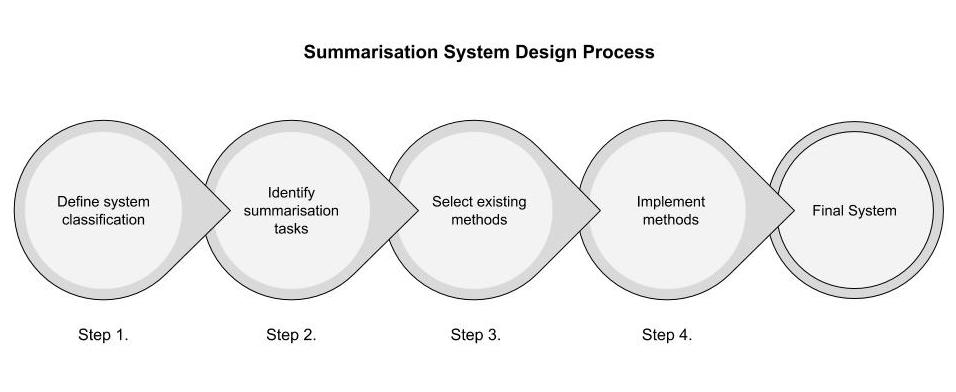
\includegraphics[width=1.0\textwidth]{Figures/Design_Process.jpg}
          \caption{Design process used for this project.}
           \label{design}
\end{figure}

\section{Requirements of The System}
To better describe the system, requirements are defined from the motivations and design objective of this project. The objective addressed in this chapter is to design a domain specific personalised summarisation system, independent of domain specific models from existing methods of extractive summarisation. The main motivation for such a system is to provide a summarisation on domains without formalised ontologies. The summarisation system purpose is to reduce information overload suffered by readers when reading multiple documents specific to a domain. From the motivation and design objective of this project the following requirements were defined for the needed summarisation system.

\textbf{R1:} The system operates on specific domain material without the use of formal supervised domain models.
\label{r1}

Summarisation systems are very good at reducing information overload as they maintain content across a set of documents while reducing the length and redundancy of which that content is discussed in the original documents. Domain specific summarisation systems produce better summaries from their comprehension of domain term relations and domain topic coherence. But these systems are often dependent on supervised models, which don’t exist for many domains of content on the internet. Thus this requirement aim is to produce a system design which performs domain specific summarisation within domains without formal ontologies. 

\textbf{R2:} The system forms summaries which significantly reduce the original content, while maintaining the most salient content, reducing the effects of information overload.
\label{r2}

Summaries best reduce information overload when they can minimise the content presented to the user without the loss of important content from the source documents. Thus in order for a system to reduce information overload it must attempt to reduce large amounts of textual content to its smallest, most salient form. Thus this specifies that this system must attempt to perform summarisation in a way that most greatly reduces original content inorder to have the best effect in reducing information overload.

\textbf{R3:} The system produces interpretable output that enhances user processing capabilities of the information being summarised.
\label{r3}

A user's ability to appropriately use a system often comes from their understanding of its operation. Providing interprobility of the system output helps a user understand why and how a summary is produced. Within a query-based system this can help a user adjust either the systems understanding or their query to better represent their information need, referred to as interactive information retrieval.  Including features of the original document from which the system used to construct a summary, allow for a summary not to act solely to inform a user but also to refer them to relevant documents which the content of the summary is presented in longer form. This is important because the usefulness of a summarisation is not solely limited to its summary readability and coverage of the source content.

\textbf{R4:} The system provides summaries which are personalised to a user's information needs.
\label{r4}
Personalisation is another method to further reduce the effect of information overload. Personalised summaries, also referred to as query-based summaries, require that the information summaries from a document set is specific to the information needed of the user. Performing a Personalised summarization is difficult within specific domains as the representation that is used must understand term relationships within a expressed query inorder to create a summary of relevant content. Thus this is required for the system as it must be able to understand term relations to allow for personalisation of summaries in a given domain.

\textbf{R5:} The system is constructed from existing extractive methods of summarisation that use topic representations as their immediate representation of source documents.
\label{r5}

Extractive methods don’t require semantic or natural language processing in the formation of the summary. Thus for the system to provide summarisation of unseen domains it must form summaries using extractive methods as they do not require supervised models for summary formation.

\textbf{R6:} The system is designed to be used with topic model based recommender systems.
\label{r6}

As discussed in the introduction one of the main motivations for this project is the similarity of constructing an extractive topic representation and automatically created ontologies, thus to serve this motivation the system should perform summarisation using a topic representation that is used in extractive summarisation. 

\section{Classifying the System}
This section presents the result of performing Step 1 of the design process. This step defines the system using a set of classifications derived from the system requirements. The classification of an automatic text summarisation system describes the system’s functionality at a high level. Preemptively defining the classification of a system, reduces the scope of methods and implementations to be considered for the inclusion in the system’s design, as well as providing a high level description of the system’s methods used to perform summarisation. In this section the classifications of automatic text summarisation are used to define the classifications of the required summarisation system. The selected classification for the system is shown in Figure \ref{fig:classification}. 

\begin{figure}[h]
    \centering
         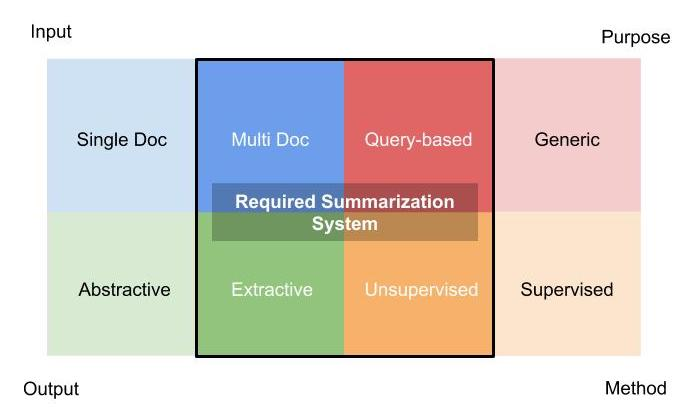
\includegraphics[width=.70\textwidth]{Figures/System_Classification.jpg}
          \caption{Classifications identified for the needed system.}
           \label{fig:classification}
\end{figure}

\subsubsection{Method: Unsupervised}
The most vital classification of the summarisation system is that the method of summarisation is unsupervised. As described by requirement \textbf{R1} of the system, the main motivation for this project is to provide a system which can provide domain specific personalised summaries without the need of supervised domain models. Such a system is required for the majority of content that exists without formal domain models. Domain ontologies are supervised even when automatically created. Inorder to design a system which is free from supervised domain models, the system must use unsupervised methods. Therefore the desired system can be classified as an unsupervised summarisation system.

\subsubsection{Input: Multi-Document}
Requirement \textbf{R2} of the system requires that textual content is reduced as much as possible to significantly reduce the effects of information overload. Summaries reduce information overload as they produce the most salient content from a document set. Inorder to best reduce the effects of information overload the summarisation the system must produce summaries from multiple documents. This also helps to satisfy requirement \textbf{R4}, as information related to a specified information need might be more likely to be spread across multiple documents then to be contained solely within a single document. Therefore the desired system can be classified as a multi-document summarisation system.

\subsubsection{Purpose: Query-based}
To satisfy requirement \textbf{R4} of the system design, the summaries produced by the system must be personalised. Personal summaries further reduce content presented to the user by considering their specific information needs. Personalised summaries are generated from an information need expressed as a query. Thus the desired system is classified as a query-based summarisation system. 

\subsubsection{Output: Extractive}
To allow for independence from formal ontologies the system must produce summaries that are created using extractive methods, satisfying requirement \textbf{R1} and \textbf{R5}. Abstractive summaries are reliant on domain semantic models, ontologies, or knowledge bases, thus extractive methods must be used so the system is independent of  supervised domain models. Extractive summarisation methods use topic representations, which are similar to ontologies. This similarity is one of the key motivations to the research question, and the system must be designed to be used with recommender systems, required in \textbf{R6}. Therefore the needed system is classified as an extractive summarisation system.

\subsection*{System Classification}
The classifications made for the summarisation system’s input, purpose, and output define the required domain independent personalised summarisation system as unsupervised, multi-document, query-based and extractive. This classification will be used by subsequent steps of the design process, to identify the necessary tasks and methods of the system.

\section{Identifying Summarisation Tasks}
This section presents the result of performing step 2 of the design process. Step of the design process identifies the tasks that the required system must perform. The tasks of a summarisation system are the operations that a summarisation system performs to produce a summary. While the tasks of a summarisation system do not directly describe the function of the summarisation systems, identifying the tasks required by a summarisation system provides an armature for which methods to perform tasks are applied.  The construction of methods from identified tasks presents the design of the summarisation system. This section identifies the tasks necessary for the system to perform to satisfy the requirements set from the design objective. The tasks identified for the required system were first derived from the universal set of tasks performed by all automatic text summarisation systems. From the universal tasks, accessory tasks were added that address the specific requirements of the desired system. The tasks identified in this section outline the operation of the proposed summarisation system in full.

As presented in Section \ref{sec:2.4} of the literature review, \citet{nenkova2012survey} define a set of tasks that are universal to extractive automatic summarisation systems. These universal tasks are:

\begin{itemize}
    \item Creation of an intermediate representation of documents.
    \item Scoring of sentences.
    \item Selection of setneces to form a summary.
\end{itemize}

From the foundation of these universal tasks, accessory tasks can be added that perform operations specific to the requirements of the summarisation system. The tasks identified for this system can be classified into tasks dependent on input document structure,  and tasks independent of docs. Both of these types of tasks exist within the system. To design a system which could be used with recommender systems (\textbf{R6}) external tasks that would be performed by a recommender system were also considered. The tasks identified are presented in Figure \ref{tasks}.

\begin{figure}[h]
    \centering
         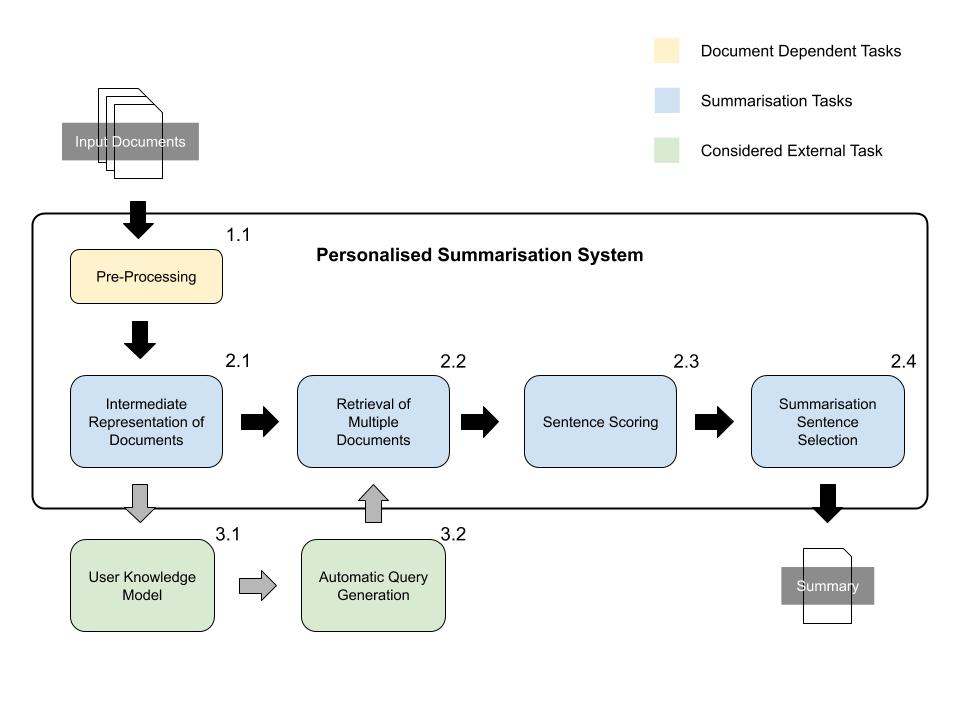
\includegraphics[width=1.0\textwidth]{Figures/Task_of_FYP_system.jpg}
          \caption{Tasks considered for the proposed system.}
           \label{tasks}
\end{figure}

\subsection{Task Group 1: Document Specific Tasks}
The tasks of this group are specific to the input documents. The aim of this task group is to prepare the raw input material to be used in the construction of the immediate representation, used in subsequent operations of the summarisation system. The method used to perform these tasks must directly address the features of the input documents, thus this task is classified as a document dependent task. In this system, the preprocessing 1.1 task is the only document specific task. Preprocessing refers to the operation of multiple methods that adjust the input material to be used in the creation of the immediate representation. Common operations performed by preprocessing tasks include: the removal of non-textual content, segmenting a document's textual content for the intermediate representation, as well as extraction of metadata from documents to be used in summary generation or in the output of the system. The method chosen to perform this task, would be altered if the type of input material was changed to a different form, such as news articles, academic journals, or social media posts. In this system the preprocessing task must address the specific operations necessary for xml structured Wikipedia articles used as input. The output from this task are textual elements extracted from the source material which allow for the intermediate representation 2.1 task to be performed.

\subsection{Task Group 2: Summarisation System Tasks}
The tasks of group 2 are tasks that are done by a summarisation system that are  independent of the source material. These tasks perform the core operations needed in producing summaries. From the classification and requirements outlined for the desired system, the operations carried out by this tasks group must serve the summarisation of multiple documents based on a personalised query. The tasks in this group have the following operations and output:

\textbf{Task 2.1}: This task creates an intermediate representation from the inputted pre processed documents. The intermediate representation of the text allows for the identification of salient sentences in the retrieval of documents task 2.2 and the scoring of sentences in task 2.3. The intermediate representation of documents has been specified by \textbf{R5} to be a topic representation, which aids in satisfying \textbf{R6} as topic representations are commonly used as well by the recommender system. Thus this task outputs representation of each document in the system as a set of topics.

\textbf{Task 2.2}: The retrieval of documents is an accessory task, not universally found in automatic text summarisation systems. The retrieval of documents task is specific to the system classification to produce query based summaries. This task uses a supplied query, from a recommender system or user, to select relevant documents. Because this system is classified as extractive, the summary is formed from document sets found relevant. Therefore the personalisation of the summary produced comes directly from the found relevant document set used in summary formation, aiding satisfying requirement \textbf{R4}. The output from this task is a subset of the input documents that have high relevance to the provided query.

\textbf{Task 2.3}: The sentence scoring task takes the sets of relevant documents and scores the sentences they contain based on the document topic representation given in task 2.1. The sentences with higher scores are those that cover the most salient material of the given document set, and thus should be prioritised for selection in the following sentence selection task. The output from this task is a set of scores from the sentences given from a set of relevant documents.

\textbf{Task 2.4}: In the summary sentence selection task 2.4 the inputted sentences and their scores are used to produce a summary of relevant material. Due to personalisation of content that is done in the document retrieval task 2.2, formation of this summary can be generalised to all the material it is given. The output from this task is a summary covering the most salient content from relevant material retrieved from task 2.2. 

\subsection{Task Group 3: External Recommender Systems Tasks}
Group 3 are tasks that are not part of the personalised summarisation system and thus were not included in the design or implementation of the system. These tasks are important to consider when selecting the methods to perform task 2.1 \& 2.2, as consideration for these tasks follows requirement \textbf{R6}, that the system should be designed to be used within a recommender system. Tasks of group 3 relate to the operations of recommender systems that would use the system's intermediate representation of documents to provide recommendations via queries. Recommender systems and user information need modeling is outside the scope of this project, but these tasks are to be considered so the summarisation system facilitates personalisation via a recommender system in possible future work.

\section{Selecting Existing Methods}
This section presents results of performing step 3 of the design process. This step produces a system design from the selection of methods to perform necessary operations of the required summarisation system, outlined by the tasks identified in Figure \ref{tasks}. The review of existing methods of extractive text summarisation in Chapter \ref{chp:2}, was used to inform the selection methods. Each task was approached by selecting a method from the existing summarisation systems. A method was selected to perform a task based on the following criteria:
\begin{itemize}
    \item The method performs well against other methods that perform the same task.
    \item The method helps satisfy one or more of the requirements outlined for this system.
    \item The method interfaces well with previously selected methods.
\end{itemize}

The methods that were examined and then selected for the system design, partially or completely fit under previously defined classifications of the system. It is important to note that the ordering in which methods are selected must respect dependencies between tasks. An example of task dependencies is the following, task 2.2 and task 2.3 are dependent on the intermediate representation method chosen for task 2.1, and the preprocessing done in task 1.1 is dependent on the intermediate representation task 2.1. The order that methods were selected for this system, respects these task dependencies. The selection of methods is presented chronologically in this section. From the selection of methods to perform a task, the methods which are selected on dependent tasks are further constrained, as they must interface with the method that was selected for a dependent task. From this process of selecting a method for each to perform the identified tasks, a design is presented which fulfills the requirements of the system thus satisfying the design objective of this project.

\subsection{Intermediate Representation}
The most important method to perform a task in the summarisation system is the method used to intermediately represent documents. This task's importance comes from the dependency of other methods that are used for the tasks of preprocessing, retrieval, and scoring are reliant on the method chosen to form the intermediate representation of documents. The methods examined to possibly perform the formation of intermediate representation were extractive summarisation methods that use topic representations, reviewed in Section \ref{subsec:2.3.1}. Extractive topic representation methods satisfy the requirement that the system is extractive as well as the requirement that the system design can be used with topic model based recommender systems. The method selected to intermediate represent documents for this system is topic model formed from the Latent Direlect Allocation (LDA) method.

\subsubsection{Latent Direllect Allocation Topic Representation}
\label{subsec:3.5.1}
Latent Direllect Allocation is an unsupervised generative probabilistic method for modeling a corpus (i.e. document set). LDA represents each document in a corpus as a probabilistic distribution over a number of latent topics. Every latent topic is made up of a probabilistic distribution over all words in the corpus. The mathematical representation of this method is as follows:

A given corpus $D$ consists of $M$ documents, document $d$ having $N_d$ words.
The model is formed from the following generative process
\begin{enumerate}[(a)]
      \item Choose a multinomial distribution $\phi_t$ for topic $t$ ($t \in \{1,\dots,T\}$) from a Dirichlet distribution with parameter $\beta$.
      \item Choose a multinomial distribution $\theta_d$ for document $d$ ($d \in \{1,\dots,M\}$) from a Dirichlet distribution with parameter $\alpha$.
      \item For a word $w_n$ ($n \in \{1,\dots,{N_d}\}$) in document $d$.
      \begin{enumerate}
            \item Select a topic $z_n$ from $\theta_d$.
            \item Select a word $w_n$ from $\phi_{zn}$
      \end{enumerate}
\end{enumerate}
In this process the words in documents are the only observed variable, while other variables are latent ($\phi$ and $\theta$) and hyper parameters ($\alpha$ and $\beta$). To infer the latent variables and hyper parameters, the probability of observed data $D$ is maxmised by (\ref{ldaUpdate}).

When an unseen or seen document is given to the model the output is a probabilistic distribution of latent topics. These probabilistic distributions can be used with metrics such as cosine similarity to determine the similarity of documents for retrieval. The formation of LDA topic models is done solely on a corpus of documents, satisfying the requirement of the system of being independent of domain specific models, \textbf{R1}. Extractive summarization methods that use LDA models for topic representations have also shown good performance for multi-document summarisation \citep{daume2006domain,wang2009multi}. When the set of documents used to create the model is a corpus of domain documents, LDA’s topic model is a representation of the term to topic relations of that domain. LDA topic models are also commonly used in user modeling in recommender systems \citep{pandit2013query, harvey2013building, mehrotra2015terms}. This common model for document representation and user understanding could be used in extending the system to perform summarisation as part of a recommendation system. LDA compared to other methods had strong performance, and satisfaction of requirements \textbf{R1, R5,} and \textbf{R6}. With LDA used as the intermediate topic representation of documents, methods for performing preprocessing, document retrieval and sentence scoring were further constrained to methods that work with a LDA intermediate representation.

\subsection{Preprocessing}
\label{subsec:3.5.2}
Preprocessing refers to the extraction of textual content from a corpus of raw documents. The textual content extracted from source documents is used by a subsequent method to create an intermediate representation. The method chosen to perform preprocessing for this system, must respect both the structure of the source content (Wikipedia articles) as well as produce an output in the form needed by the intermediate representation method, LDA. To respect the structure of input documents, methods of preprocessing were selected from existing systems that operate on news articles. Both news articles and historical Wikipedia articles are based on a singular subject and present events and explanations based on the article’s subject matter. Thus the preprocessing for news articles and historical Wikipedia articles can be assumed to be similar, based on the similarity of their content.  To produce preprocessed text in a form that respects the LDA method for performing intermediate representation, methods of preprocessing were selected from summarisation systems that also use LDA for their intermediate representation. Combining methods of preprocessing from similar systems produces a method of preprocessing for this system that respects both the input documents and the intermediate representation of this system.

\subsubsection{Text Normalisation}
Natural text is presented in a form that is readable to humans. Text normalisation is the process of transforming natural text to a form that is more readable to a machine. Text normalisation is a common task in natural language processing. Text normalisation cleans the raw natural text to be better used in creation of a LDA topic representation of a document's content. Text normalisation methods to be used for LDA are the conversion of all words to lowercase, removing punctuation, removing of stopwords, expanding abbreviations, and canonicalization of words. These steps are standard and are produced by most systems that use LDA.

\subsubsection{Article Representation}
Identifying the structure of the input documents helps to determine how textual content should be inputted into the method used for the intermediate representation. In this project the input documents to be used for summarisation are 32 Wikipedia articles related to the Watergate Scandal. Wikipedia articles use an encyclopedic style to present information relating to a specific topic. Wikipedia articles present information in a structure where each paragraph discusses a topic in a specific context. It is important to note that LDA has been shown to have better accuracy when performed on a large corpus set \citep{crossley2017important}. The corpus used for this system is relatively small. In an attempt to increase accuracy and to construct a model that is representative of the paragraph styling of Wikipedia articles, each paragraph in an article was treated as a separate document. This hopes to improve performance that would otherwise be suffered from treating each article as a separate document. Metadata from a document source article, such as the title and url, is also maintained to be used in explanation of the system generated summary. This helps with satisfying requirement \textbf{R3} of the system, by enhancing user processing of summary information via references to the articles from which the extractive summary was formed from.

\subsubsection{Concept Extraction}
Extractive summarisation systems that process similar documents to the Wikipedia article for use in a LDA topic representation were examined to select a method to perform preprocessing for this system. The original implementation of LDA uses a bag-of-words representation to create a topic model \citep{blei2003latent}. Recent work on news article summarisation systems that use LDA, have found better summarisation performance by using a bag-of-concepts representation of document content \citep{rajagopal2013commonsense,li2016cross,raviv2016document}. A bag-of-words representation treats each document as a list of sentences, where each sentence is a list of words contained in the corresponding sentence. A bag-of-concepts changes out the sentence list to contain concepts of a sentence rather than words. For each sentence a list of concepts is created. A Part of Speech Tagger is used to tag words with their parts of speech (POS) in each sentence. Word pairs are extracted from a tagged sentence by selecting specific POS, such as verb noun pairs, nouns, and named entities. The word pairs are then normalised into concepts by centralising terms into common meaning, via a semantic model. These normalised word pairs are the concepts that make up a list which sentence is represented by. For example the sentence “Vice President Gerald Ford succeeded to the presidency upon Nixon's resignation.” is represented in the POS dependency tree in Figure \ref{pos}. 

\begin{figure}[h]
    \centering
         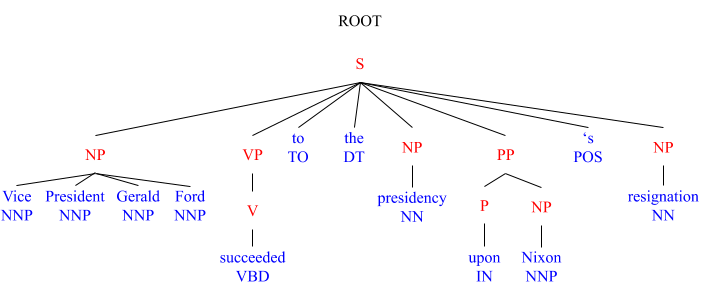
\includegraphics[width=1.0\textwidth]{Figures/POS_TREE.png}
          \caption{POS dependency tree for "Vice President Gerald Ford succeeded to the presidency upon Nixon's resignation".}
           \label{pos}
\end{figure}

The dependency tree is traversed to extract necessary POS to represent concepts. An example of this is the extraction of such as a noun pair (NP), n-gram pairs of nouns referring to a single object. The extracted noun pairs from this example would be: “Vice President Geral Ford”, “presidency”, “nixon” and “resignation”.

The bag-of-concept representation achieves better performance than the traditional bag-of-words representation. The performance of the LDA is increased by reducing the noise in the LDA topic model that occurs when unimportant words from the text are used in the topic word distributions. The bag-of-words representation treats all words as independent, disregarding dependencies between words. The bag-of-concept representation attempts to respect the dependence of words, resulting in an improvement in the accuracy of the model in representing the source content, as well as limiting noise by only including the most representative word grouping of a sentence’s meaning.

The method chosen for this system is a stripped down approach to other bag-of-concept document representation implementations. The stripped down approach was taken to avoid the use of semantic models to normalise extracted concepts. The method selected for the system extracts just noun pairs and named entities. A semantic model is not used to centralise concepts. The method therefore treats the extracted concepts: “president nixon”, “richard nixon” and “nixon” independently. This simpler approach was done in an attempt to build the summarisation system with no reliance on semantic models, satisfying requirement \textbf{R1}. Without centralising concepts the LDA model accuracy is expected to be reduced compared to a model built with normalised concepts, but this method should provide better performance compared to traditional bag-of-concept methods of preprocessing. 

\subsection{Document Retrieval}
\label{subsec:3.5.3}
The method selected to perform the retrieval of multiple documents utilizes the intermediate representation of all documents to produce a subset of documents that are relevant to a given query. The set of relevant documents is used for the scoring and summarisation tasks of the system to produce an extractive summary. The system’s ability to personalise summaries comes from how well the system can determine a users information need from a query and how well the system is able to find documents that satisfy that information need. To address these factors document retrieval was broken up into two processes. The first process is a method for which a given query is expanded. Query expansion is a common method performed in information retrieval. Query expansion reduces the number documents found relevant from adding terms to the query. Additional terms further specify information needed for the query making it more specific. The second process is the method in which a query is used to retrieve relevant documents. Together these processes form the method used for retrieving documents relevant to a query.

\subsubsection{Process 1: Query Expansion}
Query expansion is a common information retrieval task. Queries are expanded by taking an original query and adding content to it based on the system's interpretation of the queries meaning. Expansion increases the performance of document retrieval by limiting document and query mismatching \citep{carpineto2012survey}. Due to this being reliant on the systems interpretation of document content, methods that attempt to expand queries using a LDA topic model presentation were examined. 

The method chosen for performing query expansion is proposed by Li and Jin’s \citeyear{li2016cross} paper “Cross-document knowledge discovery using semantic concept topic model.” In \emph{2016 15th IEEE International Conference on Machine Learning and Applications (ICMLA)}. The method they present forms concept chain queries, which attempt to detect links between two topics of interests across documents. Given a query that contains concept A and concept C, this method uses the topic representation to determine the path between concept A and C, expanding the query with the inclusion of intermediate terms of concept B. The algorithm for the method is as follows:

\begin{enumerate}
    \item Conduct an independent search for concept A and concept C, and collect relevant sentences in which A and C appears. These sentence sets are defined as AS and CS;
    \item Union set AS and CS to form a new document collection. This new set is the relevant context for the query pair A and C and is used in the subsequent topic discovery sent, this set is referred to as BS;
    \item Apply LDA model on BS and generate topically relevant terms for A and C. The generated terms are constrained to concepts appearing in the original dictionary of the LDA model;
    \item For each topic determined by the model on set BS identify top semantic concepts, which serve as B level terms connect A and C topically;
\end{enumerate}

A query given by a user might contain two domain terms that are not closely related. With systems that use domain models this is easily handled, as ontologies or semantic models can be traversed to find a common parent concept or term. The method selected for query expansion emulates an ontology based approach by smoothing conceptual jumps by adding terms that have common relationships to the domain concepts presented in the original query. Since the system produces an extractive summary directly from the documents relevant to a query, the expanded query from this method should produce documents that link logical jumps in the original query, producing a summary that is able to connect logical jumps of domain specific terms. 

\subsubsection{Process 2: Query-Based Retrieval}
The goal of query based document retrieval is to produce a set of relevant documents based on a given query. This is approached by scoring all documents for their relevance to a given query and then selecting the n-most relevant documents as an answer. The scoring for relevance has many approaches, and is its own field within computer science. Many methods exist that use LDA query based document retrieval. The LDA topic model can produce a topic distribution for an unseen document. Thus LDA can be used for assessing the topic distribution of a given query and then determining documents that are relevant to that topic distribution. The output from passing a query to the LDA model is the probability of topics that query relates to based on the words that a query contains. With the same topic distribution given for documents the probability of producing a given query given a document can be determined. Documents that produce higher probabilities of producing the given query are then treated as more relevant. Methods that directly use the LDA topic model probabilities, heavily rely on the accuracy of the topic model. Due to the small corpus size used in designing this system, the LDA topic model formed from the corpus is more susceptible to inaccuracy \citep{crossley2017important}. Other LDA based approaches for retrieval use the topic distribution of documents and query to calculate similarity. Highly similar documents to query are then treated as relevant \citep{steyvers2007probabilistic}. These methods are not as direct as using direct probabilities, and therefore are less reliant on the accuracy of the model. Therefore The method chosen for retrieval in this system is the cosine similarity of a document topic distribution and a query distribution.

When a query is given to the system, all of the documents are scored based on the cosine similarity \ref{cosim} of the document’s topic distribution at the topic distribution of the query. When a document, a wikipedia article or user query, is input into the LDA model, a vector of topic ids and corresponding weights are given. Cosine similarity can be calculated as follows:

Consider the two topic distributions $\vec{Q}$ for query and $\vec{D}$ for document. Each contains $k$ probabilities of them relating to each of the $k$ topics in the topic model. The similarity of the distributions can be calculated by:
\begin{equation}
    cossim(\vec{Q}, \vec{D}) = \frac{\sum_{i=0}^k q_i \times d_i}{\sqrt{\sum_{i=0}^k q_i^2}\sqrt{\sum_{i=0}^k d_i^2}}
    \label{cosim}
\end{equation}
All documents are scored against a query and the documents selected to be relevant are those with a similarity above a specified threshold. LDA is not the best used method for document retrieval. \citet{wei2006lda} present that LDA itself is too coarse of a representation to be used as the sole representation for document retrieval. Considering this is a component of a larger system using the LDA topic model for retrieval is sufficient, as it interfaces well with the existing LDA topic representation of the system.

\subsubsection{Document Retrivel Method: Process 1 \& 2}
The method used for the retrieval of multiple documents from a query is as follows. For each imputed query, it is expanded with terms that relate to its topic representation, then all documents are scored based on their cosine similarity with the expanded query. Documents are returned if their similarity is above a threshold. This method results in a document set to be used in the formation of a summary. The summary is personalised from the query relevant content found relevant based by this method. 

\subsection{Sentence Scoring and Summary Selection}
label{subsec:3.5.4}
Sentence scoring is used in the selection of document sentences for a summary. The aim of sentence scoring in extractive summarisation is to score sentences in respect how well they cover the content of the documents being summarised. These scored sentences are then used in a method which selects  sentences based on their scores to form a summary. For both these tasks are implemented via a method that includes the scoring and selecting of sentences as one. The method chosen for sentence scoring as well as sentence selection is the method presented by Alguliev et al. \citeyear{alguliev2011mcmr} “MCMR: Maximum coverage and minimum redundant text summarization model” in \emph{Expert Systems with Applications}. The method presented by Alguliev et al, outperforms other methods of performing extractive summarisation \citep{gambhir2017recent}. This method is also unsupervised and requires no other representation or pre processing of textual content. Thus this method was easily identifiable as the method to perform sentence scoring and summary generation for the required system.

\subsubsection{Sentence Selection}
Considering a document collection $D = \{d_1,d_2,\dots, d_{|D|}\}$ where $|D|$ is the number of documents. Each document contains a set of sentences $d_i = \{s_1,s_2,\dots,s_{|d_i|}\}$ where $|d_i|$ is the number of sentences in the ith document. This method considers the document collection as a set of all sentences $D = \{s_1,s_2,\dots,s_n\}$ where $s_i$ is the ith sentence in document collection $D$ and $n$ is number of sentences in the document collection. $T = \{t_1,t_2,\dots,t_m\}$ represents all the terms occurring in $D$, where $m$ is the number of different terms. The method attempts to find the subset of the sentences  $D = \{s_1,s_2,\dots,s_n\}$ that covers the main content in the document collection. $S$ be the set of sentences constituting a summary, the similarity between the document collection and the summary is $sim(D,S)$, which is what is going to be maximised. The length of a desired summary is used as a cardinality constraint on the maximisation of $sim(D,S)$, so that summary is of length $L$ or shorter, where $L$ is a number of words in the summary. This formalises the summarsation problem as follows:
\begin{equation}
    Maximise \; sim(D,S) \\
    s.t. \; len(S) \leq L
    \label{mcmrSimple}
\end{equation}

This alone does not minimise the redundancy in the produced summary. Thus the following formalisation is used. 

Let $x_{ij}$ denote a variable which is 1 if the pair of sentence $s_i$ and $s_j$ are selected to be in the summary, otherwise 0, and $len(s_i)$ denote the length of sentence $s_i$. Thus assuming that each sentence is a candidate summary sentence the problem can be written as:
\begin{equation}
    Maximise \: f = \sum_{i=1}^{n-1} \sum_{j=i+1}^n [sim(\vec{D}, \vec{s_i}) + sim(\vec{D}, \vec{s_j}) - sim(\vec{s_i}, \vec{s_j})]x_{ij}
    \label{mcmrGeneral}
\end{equation}
\begin{equation}
    s.t. \; \sum_{i=1}^{n-1} \sum_{j=i+1}^n [len(s_i) + len(s_j)]x_{ij} \leq L
    \label{mcmrConstraint}
\end{equation}
\begin{equation}
    x_{ij} \in \{0,1\} \forall i,j
    \label{mcmrVar}
\end{equation}

Now the objective is to find the binary assignment on $x_{ij}$ with the highest score,best coverage and least redundancy, such that summary length is at most $L$. This formation is an integer linear programming problem where both the object function and constrained at the linear set of integer variables. The object function guarantees that the produced summary will be covered by the summary from the first and second terms in \ref{mcmrGeneral}. The third term also guarantees that the summary will not contain multiple sentences that convey the same information, reducing redundancy. The integrality constraint on $x_{ij}$ is automatically satisfied in \ref{mcmrVar}.

\subsubsection{Sentence Scoring}
This system uses two scores for sentences and the score of a sentence is a weighted sum based on a specified alpha value. The two scoring metrics are a cosine similarity of TF-ISF (Term Frequency, Inverse Sentence Frequency) scores of terms in a sentences and the Normalised Google Distance. 

\textbf{Cosine Similarity of TF-ISF}
Each sentence is represented as a vector of weighted terms given by their TF-ISF scores. $s_i =\{w_{i1};w_{i2}; \dots; w_{im}\}$ where $m$ is the number of terms in the document collection, $w_{ik}$ is the weight of term $t_k$ in the sentence $s_i$. The element $w_{ik}$ is defined using the TF-ISF, given in \ref{tfisf}.
\begin{equation}
    w_{ik} = f_k \times \log(\frac{n}{n_k})
    \label{tfisf}
\end{equation}
Where $f_k$ is the term frequency the number of occurence of term $t_k$ in sentence $s_i$, $n_k$ denotes the number of sentences in which $t_k$ appears and $n$ is the number of sentences. The $\log(\frac{n}{n_k})$ is referred to as the isf factor. TF-ISF assigns a weight to term $t_k$ in a sentence $s_i$ that is:
\begin{enumerate}
    \item Highest when $t_k$ occurs many times in a small number of sentences;
    \item Lower when a term occurs few times in a sentence, or occurs in many sentences;
    \item Lowest when the term occurs in virtually all sentences;
\end{enumerate}

From the vectors of weights for each term in two sentence, $\vec{s_i}$ $\vec{s_j}$, the cosine similarity is calculated.
\begin{equation}
    sim_{cos}(\vec{s_i},\vec{s_j}) = \frac{\sum_{k=1}^m w_{ik} w_{jk}}{\sqrt{\sum_{k=1}^m w_{ik}^2}\times\sqrt{\sum_{k=1}^m w_{jk}^2}}, i,j=1,\dots,n
    \label{cossimSent}
\end{equation}


\textbf{NGD-Based Similiary}
To calculate normalised google distance similarity each of sentence is represented by a list of terms. $s_i=\{t_1,t_2, \dots, t_{|s_i|}\}$ where $|s_i|$ is the number of distinct terms in sentence $s_i$. The similarity of sentences $s_i$ and $s_j$ can be calculated using:
\begin{equation}
    sim_{NGD}(s_i, s_j) = \frac{\sum_{t_k \in s_i} \sum_{t_l \in s_j} sim_{NGD}(t_k,t_l)}{|s_i| \times |s_j|}, \\ where \; sim_{NGD}(t_k,t_l) = \exp(-NGD(t_k, t_l))
    \label{ngdSent}
\end{equation}

\begin{equation}
    NGD(t_k,t_l) = \frac{max\{\log(f_k), \log(f_l)\}-\log(f_{kl})}{\log n - min \{\log(f_k),\log(f_l)\}}
    \label{ngdTerm}
\end{equation}
Where $f_k$ is the number of sentences term, $t_k$ appears in, $f_kl$ is the number of sentences both $t_k$ and $t_l$ appear in, and $n$ is the number of sentences in the document collection.

These similarity measures are both used making the true formula for MCMR summary formation the following.
\begin{equation}
    Maximise \: f_{\alpha} = \alpha \times f_{cos} + (1-\alpha) \times f_{NGD},
    \label{mcmrFull}
\end{equation}
$where$
\begin{equation}
    f_{cos} = \sum_{i=1}^{n-1} \sum_{j=i+1}^n [sim_{cos}(\vec{D}, \vec{s_i}) + sim_{cos}(\vec{D}, \vec{s_j}) - sim_{cos}(\vec{s_i}, \vec{s_j})]x_{ij}
\end{equation}
\begin{equation}
    f_{NGD} = \sum_{i=1}^{n-1} \sum_{j=i+1}^n [sim_{NGD}(\vec{D}, \vec{s_i}) + sim_{NGD}(\vec{D}, \vec{s_j}) - sim_{NGD}(\vec{s_i}, \vec{s_j})]x_{ij}
\end{equation}

\subsection{System Design with Methods}
With the methods selected to perform each of the identified tasks, the design in Figure \ref{designD} is constructed. The design represents four main processes of the system, each of which are  performed from the selected methods of this section. This design can also then be compared directly to the original requirements outlined for the system, to determine if it achieves the requirements necessary to achieve the design objective of this project.

\begin{figure}[h]
    \centering
         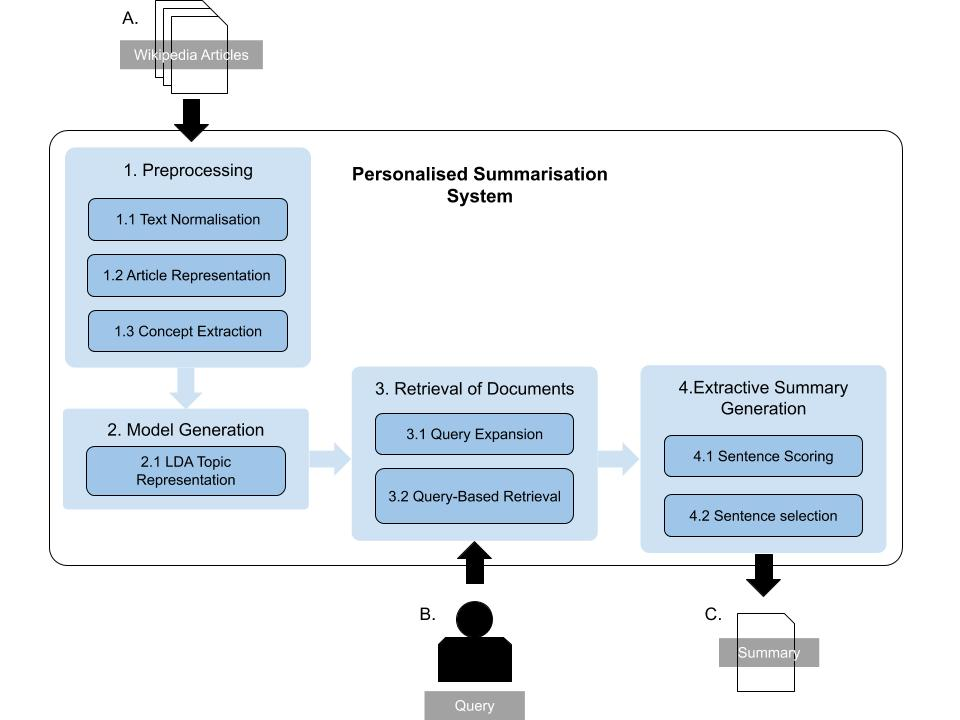
\includegraphics[width=0.80\textwidth]{Figures/System_Design_from_Design_Chapter.jpg}
          \caption{Design developed from the classification, tasks, and methods identified for the needed system.}
           \label{designD}
\end{figure}

The four processes in the system design are Preprocessing, Model Generation, Retrieval of Documents, and Extractive Summary Generation. These processes are constructed from the methods selected to perform the identified tasks needed by the system. Together their functionality explains the functionality of the proposed Personalised Summarisation System. Preprocessing includes the methods used for identified tasks of preprocessing. These methods include text normalization, article representation and concept extraction. From the Preprocessing process a bag-of-concepts representation is constructed from the raw Wikipedia article input. The bag-of-concepts is used in the Model generation process which uses the LDA method to create a topic model of all content in a domain. This topic model is used in the Retrieval of Documents, to expand a given query and then assess document similarity from the domain set of documents to produce a set of relevant domain documents related to a query. The set of relevant documents is then used in the Extractive Summary Generation Process. Here the sentence scoring and sentence selection methods find the most salient sentences from the retrieved documents and extractive summary is produced. The design addresses and satisfies all of the requirements outlined for the needed system.

\textbf{R1:} The system operates on specific domain material without the use of formal supervised domain models.

The design uses no supervised models for either the modeling of a domain or in producing a summary. Certain methods, such as concept extraction, were modified from their original implementations to be independent of supervised models. The LDA topic representation can model a domain when given a complete set of documents that describe the domain providing system understanding of domain terms and their relationships as topics. Lastly the use of query expansion can smooth domain topic jumps that exist within a query, achieving similar functionality to supervised domain models, while being unsupervised. Thus the system here is designed to operate on domain material without the used of supervised models.

\textbf{R2:} The system forms summaries which significantly reduce the original content, while maintaining the most salient content, reducing the effects of information overload.

The personalised retrieval of documents used in forming an extractive summary greatly reduces the effects of information overload, by not only limiting information presented  to a user to be most relevant to their information need, but by also producing a summary which presents the most salient content of those retrieved documents in a short digestible form. Thus this system takes a two fold approach to limiting information overload, by reducing content to a small set of most relevant documents to a query and then producing a summary from the relevant document that maximises its coverage of material in the relevant document. This approach significantly reduces the effects of information overload, and thus satisfies this requirement.

\textbf{R3:} The system produces interpretable output that enhances user processing capabilities of the information being summarised.

In the Preprocessing process, all sentences to document and document to article relationships are maintained. With the summary these relationships can be given to a user to provide the articles in which sentences originated from in the summary. Other components lend themselves to providing interpretable output, such as the expanded query created in the document retrieval process. The expanded query identifies additional concepts which are related to concepts in the query, giving the user an understanding of the system’s interpretation of their query. The user can then adjust their query based on the system's presented interpretation allowing for the user to adjust their query to better address the true information need known as interactive information retrieval. The system methods allow for additional output to be provided which help give interpretability to an end user. 

\textbf{R4:} The system provides summaries which are personalised to a user's information needs.

The design provides personalised summaries, from producing summaries from a document set that are relevant to a given query. A given query specifies an information need, which the system satisfies by providing relevant documents from the corpus that are similar to the expressed information needed. These documents are then used in the formation of an extractive summary. Because the summary is produced from a personalised set of relevant documents itself is thus personalised to the information needed in a query.

\textbf{R5:} The system is constructed from existing extractive methods of summarisation.

Every method contained in this design was selected from systems or methods that were classified as extractive. So not only does the method for producing a summary produce them  extractively, it is supported by other methods that enhance the extractive summary formation. 

\textbf{R6:} The system is designed to be used with topic model based recommender systems.

The system uses a LDA topic representation. This representation is also commonly used by the recommender systems, to model user knowledge or interest. Thus a recommender system could share the intermediate representation of documents to produce information needs as queries. Thus the system is easily housed within a recommender system.

This design satisfies the requirements presented at the beginning of this chapter, thus satisfying the design objective of this project. Through implementation of this design the system can be assessed to determine the extent that existing automatic extractive summarization methods can be used to provide domain specific personalised summaries, independent of domain specific ontologies and semantic models.

\section{Summary of Design}
This section presented the process in which the review of automatic text summarisation literature was used to construct a domain specific personalised summarisation system, that does not require use of superived domain specific models. First a set of requirements for the system were outlined using the design objective and motivations of the project. Then the first 3 steps of the 4 step design process were completed to produce a system design that satisfies the outlined requirements, therefore producing a system that satisfies the design objective of the project.  First the classification of the system was defined. This provided a description of the  system’s functionality at a high level and grounded it within the field of automatic text summarisation. The classification of the system was then used to identify tasks to be performed by the summarisation system, identified from systems with similar classifications. Then methods were selected based on its performance, satisfaction of requirements, and compatibility with other selected methods for system tasks. With all methods selected a system design was constructed which was assessed against the requirements set at the beginning of this chapter. The design satisfied all of the requirements set and thus the presented design satisfies the design objective of this project of using existing automatic text summarisation methods to design a domain specific personalised summarisation system, that does not require use of superived domain specific models. The design produced in this chapter is used in the following chapter to implement this system, to then assess the proposed system in regard to this project's research question.